\section{Desarrollo e Implementación}
  \subsection{Descripción de la implementación}    
    Principalmente la implementación se realizó utilizando técnicas como TDD y Refactor, además de utilizar ciertos conceptos de programación orientada a objetos y programación funcional.

    Después de definir las acciones que iban a realizar los objetos que iban a interactuar con el sistema se procedió a determinar los posibles valores de entrada y salida de las mismas, concepto ampliamente usado en TDD. Las pruebas fueron pensadas tomando en cuenta los distintos elementos del ecosistema, a continuación se muestra una lista de las pruebas realizadas:

      \begin{itemize}
        \item{\textbf{AnimalsTest}}
          \begin{itemize}
            \item{Morir por falta de puntos de vida}
            \item{Beber agua considerando la fuente más cercana.}
            \item{Reproducción de un nuevo animal.}
            \item{Moverse a un nuevo lugar considerando Agua/Comida/Depredadores}
            \item{Moverse a un nuevo lugar considerando la información de algún vecino dentro del rango de visión}
            \item{Comer considerando la fuente de comida más cercana.}
          \end{itemize}
        \item{CorpseTest}
          \begin{itemize}
            \item{Decrementar la vida de los elementos cercanos al cadaver}            
            \item{Generar plantas de forma aleatoria después del tiempo de vida del cadaver.}
          \end{itemize}
        \item{NatureElements}
          \begin{itemize}
            \item{Generar un mundo dada una imagen en formato PNG y colores definidos}
            \item{Generar "n" carnívoros, herbívoros, carroñeros y cadáveres de forma uniforme en un mapa.}
            \item{Convertir una planta que carece de puntos de vida en un trozo de tierra.}
          \end{itemize}
      \end{itemize}      
    
    Todas las pruebas cuentan con un mapa de prueba generado por imagenes definidas o bien como valores de entrada del mismo desarrollador. Las pruebas pueden encontrarse dentro de la carpeta \textit{Practices/src/test/}, donde se describen con máś detalle.

    Se consideró que todos los animales contaban con el mismo comportamiento, ya que las acciones son similares en todos ellos, es por eso que se decidió usar una clase que implementa todas las acciones de forma genérica, de la cual las clases que definen a los herbívoros, carnívoros y carroñeros sobreescribieran, sólo si era necesario, los métodos y su respectiva lógica.

    Considerando el trabajo previo realizado con el juego de la vida y la regla de difusión, la adaptación de la lógica del MicroMundo fue relativamente sencilla gracias al uso de Traits (Nativos del lenguaje Groovy) e implementación de polimorfismo. La estructura (propiedades y métodos) del Trait de WorldElement se define a continuación:

    \begin{itemize}
        \item{\textbf{Propiedades}}
          \begin{itemize}
            \item{\textit{alive}: Indica el estatus del objeto, vivo o muerto.}            
            \item{\textit{life}: Indica los puntos actuales de vida del objeto en cuestión.}
            \item{\textit{sightRange}: Rango de visión (Definido por las reglas del micromundo).}
            \item{\textit{position}: Ubicación en el plano x,y.}
            \item{\textit{type}: Indica el tipo de objeto, útil para el cambio de estados.}
            \item{\textit{worldCopy}: Referencia al objeto actual del mundo, se utiliza para fines de exploración.}
            \item{\textit{nearInformation}: Dentro de un objeto de tipo llave-valor indica qué elementos puede visualizar dentro de su rango.}
            \item{\textit{canonicalName}: Nombre del objeto indicando paquete y nombre de la clase, útil para la generación dinámica de objetos con comportamientos distintos.}
            \item{\textit{operations}: Instancia del objeto operations, éste objeto define arreglos con el orden de ejecución y métodos de utilería general.}
          \end{itemize}
        \item{Métodos}
          \begin{itemize}            
            \item{\textit{decreaseLife}: Realiza el decremento de la vida dado un valor.}
            \item{\textit{increaseLife}: Realiza el aumento de la vida dado un valor.}
            \item{\textit{die}: Método que ejecuta cierta acción cuando el animal muere, se sobreescribe dependiendo el animal.}
            \item{\textit{drink}: Ejecuta la acción de beber agua considerando fuentes cercanas.}
            \item{\textit{eat}: Ejecuta la acción de comer, se sobreescribe dependiendo el animal.}
            \item{\textit{locationInformation}: Ejecuta una inspección visual del animal, actualiza el campo de nearInformation para poder consultar los datos dentro de su rango de visión.}
            \item{\textit{move}: Ejecuta la acción de moverse, es aleatoria la razón.}
            \item{\textit{moveWithInformation}: Ejecuta la acción de moverse, considerando la información que el vecino más cercano tiene, la razón es aleatoria.}
          \end{itemize}        
      \end{itemize}
    Además de llevar el control de forma dinámica de las acciones que realizarán los elementos que se encuentran dentro del mundo de prueba, también es necesario gestionar las acciones propias de éste.

    Para ello se utiliza una convención semejante, definiciendo un Trait nuevo llamado \textit{MicroWorldAutomata} donde se lleva el control de los automatas (elementos del vecindario). Cuenta con una tarea única llamada \textit{task} donde se define la lógica del recorrido de los elementos del mapa y ejecucion de las acciones pertinentes. A continuación se define la estructura de dicho Trait:

      \begin{itemize}
        \item{\textbf{Propiedades}}
            \begin{itemize}
              \item{\textit{rows}: Indica el número de filas que tiene el vecindario.}
              \item{\textit{columns}: Indica el número de columnas que tiene el vecindario.}
              \item{\textit{start}: Bandera que indica si el proceso del ejecución ha comenzado.}
              \item{\textit{operation}: Instancia del objeto operations, éste objeto define arreglos con el orden de ejecución y métodos de utilería general.}
              \item{\textit{world}: Arreglo de dos dimensiones donde se encuentran los animales y elementos del ecosistema definido.}
              \item{\textit{statistics}: Lleva el conteo de los elementos activos dentro del mapa, considera agua, plantas, carnívoros, herbívoros, carroñeros, cadáveres y tierra.}
              \item{\textit{currentElements}: Guarda la referencia de cada tipo de dato en una lista para posteriormente poder dibujarla, interactua de forma directa con la interfáz gráfica.}
            \end{itemize}
          \item{Métodos}
            \begin{itemize}            
              \item{\textit{init}: Método que se encarga de inicializar variables como rows, columns y world.}
              \item{\textit{task}: Implementación de la lógica que implica el recorrido de los elementos del vecindario y el orden de las acciones a realizar.}            
            \end{itemize}        
      \end{itemize}
    El método task es de gran utilidad debido ya que nos permite contemplar trabajo a futuro sin modificar del todo la lógica existente, bastaría con generar un objeto que haga uso de las funcionalidades del trait y definir las funciones y razonamientos necesarios.

    \begin{figure}[h!]
      \centering
        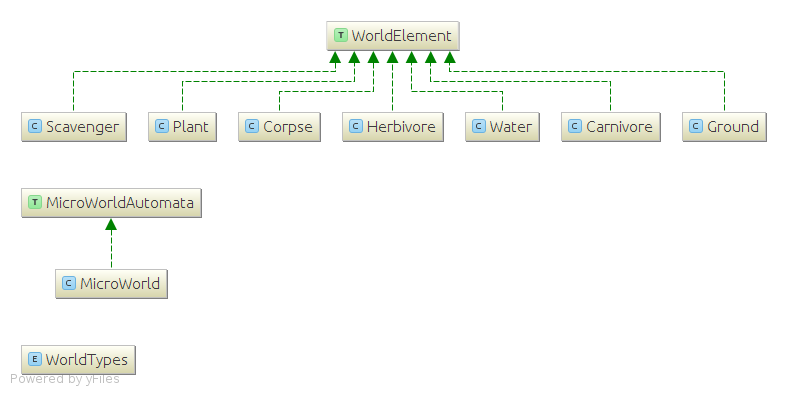
\includegraphics[scale=0.6]{./images/classDiagram}
        \caption{Diagrama de clases del MicroMundo.} 
    \end{figure}
  \newpage
  \subsection{Tecnologías}
    Se hizo uso del control de versiones Git en conjunto con su plataforma distribuida Github. Todos los códigos fuentes del proyecto pueden ser visualizados en línea a través de la siguiente liga: \url{https://github.com/jresendiz27/ComplexSystems}, dentro del mismo respositorio también se encuentran las instrucciones para poder ejecutar algun proceso, tanto del Juego de la Vida, Regla de Difusión o la simulación del MicroMundo. Las tareas que pueden ser ejecutadas fueron definidas desde Gradle.

    Gradle es otro elemento importante para el desarrollo de éste proyecto, ya que es el encargado de generar la estructura del proyecto, llevar el control de las dependencias y ejecución de tareas definidas por el usuario como; la visualización de los simuladores, el proceso de obtención de estadísticas e inserción a base de datos (Juego de la Vida y Regla de Difusión) por citar algunos.

    Se optó por realizar el trabajo usando un lenguaje multiparadigma y políglota como lo es \textbf{Groovy}. Groovy es de tipado débil y multiparadigma (Funcional y Orientado a Objetos) que se compila hacia código objeto de Java y se ejecuta sobre la JVM (Máquina Virtual de Java), es decir, cuenta con una gramática y semánticas distintas al lenguaje Java pero puede ser utilizado siguiendo las mismas normas. Esto nos trae como mayor ventaja la compatibilidad con otros sistemas que implementan o usan la JVM, además de la reutilización de bibliotecas que sólo fueron desarrolladas para Java.

    Groovy es usado durante todo el desarrollo del proyecto; debido a que la estructura del lenguaje ayuda a la generación de códigos descriptivos y menos extensos. Groovy implementa muchas operaciones con colleciones (List, Set, Map) de forma nativa sin necesidad de generar código muy extenso para poder iterar o recorrer éstas. También nos provee la ventaja de hacer uso de ciertos conceptos de programación funcional como funciones de primer orden, lambdas y closures.

    Cabe destacar que es necesario contar con Java en su versión 6 o superior para la ejecución del proyecto. Además de definir ciertos parametros en nuestras variables de entorno para que la JVM pueda gestionar mejor los recursos y poder visualizar de forma correcta los simuladores. Las variables de entorno necesarias se encuentran definidas en el archivo \textit{opts.sh} justo en la raíz del repositorio.

    El proyecto funciona siempre y cuando se le asigne un mapa (imagen llamada Sample.png, ubicada en el escritorio). Esta imagen ayudará a generar el mapa. La imágen debe tener 320 de ancho y 200 de alto; además de contener ciertos tipos de colores para las plantas, agua y tierra con los siguientes códigos hexagesimales.
      \begin{itemize}
        \item{\textit{Plantas}: 00FF00}
        \item{\textit{Tierra}: FFDEAD}
        \item{\textit{Agua}: 0000FF}
      \end{itemize}
      \begin{figure}[h!]
        \centering
          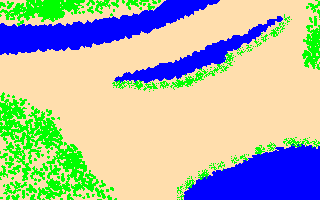
\includegraphics[width=\textwidth]{./images/Sample.png}
          \caption{Ejemplo del archivo Sample.png.} 
      \end{figure}
    Este archivo es indispensable, ya que también es usado para el proceso de generación de estadísticas. Las estadísticas se guardan en el escritorio y en un formato CSV, para que puedan ser visualizadas por Excel o de LibreOffice.
\newpage
  \subsection{Capturas de pantalla} 
    La interfáz gráfica del proyecto fue desarrollada usando Java Swing. Para el proceso de dibujado se utilizó Java2D, generando el mundo y realizando el proceso de pintado de cada elemento nuevo dentro del sistema. Por defecto el sistema carga el archivo Sample.png y lo llena con animales de forma aleatoria y uniforme tomando una distribución al 5\% del espacio libre del mundo.
    \linebreak
    \begin{figure}[h!]
      \centering
        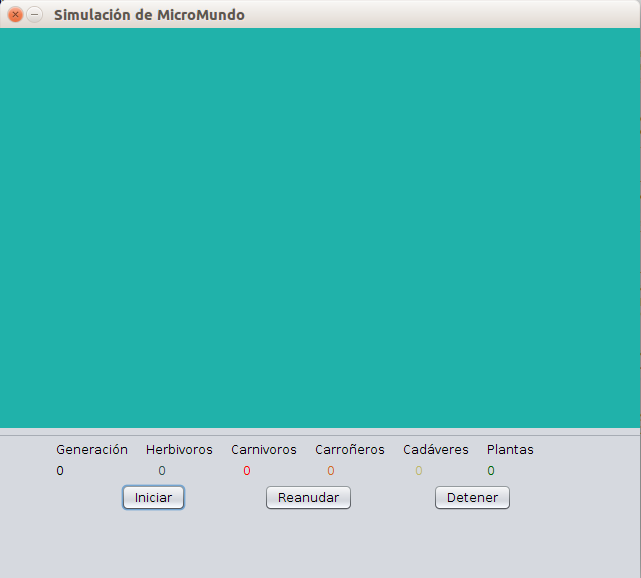
\includegraphics[scale=0.4]{./images/MicroWorldSwingInterface.png}
        \caption{Interfáz del simulador del micro mundo.} 
    \end{figure}
    \linebreak
    Los tres botones son las acciones que pueden ser realizadas durante la ejecución del simulador. Al iniciar la simulación se carga el achivo Sample.png ubicado en el escritorio y se ejecuta cada ocho segundos la lógica y dibujado del mundo. 

    Además tambien pueden verse las estadísticas actuales del mundo, tomando en cuenta la cantidad de Carnívoros, Cadáveres, Carroñeros, Herbívoros y Plantas, todo esto se obtiene por cada generación que pasa.
    \linebreak
    \begin{figure}[h!]
      \centering
        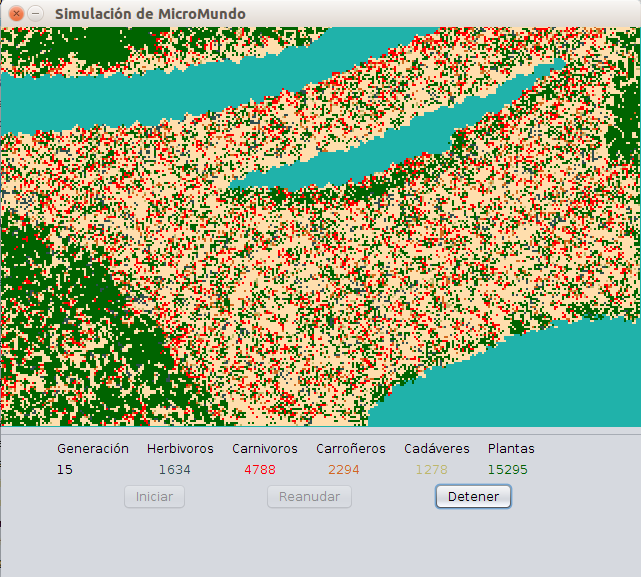
\includegraphics[scale=0.4]{./images/MicroWorldProcess.png}
        \caption{Ejecución y dibujado del MicroMundo.} 
    \end{figure}
    \linebreak
    Se tomó en cuenta el tamaño para la visualización del MicroMundo, es por ello que dentro del proceso de dibujado se escala la imágen original al doble para que pueda ser vista sin mayor problema. 

    La interfáz gráfica puede ser visualizada en ejecución desde la siguiente liga: \url{https://www.youtube.com/watch?v=AvsQTAi9elI}. 

    Se realiza una ejecución por 300 generaciones y claramente se puede visualizar el comportamiento emergente de las especies, al buscar siempre fuentes de agua y reunirse en manadas. 